Konvolūcijas slāņus plaši izmanto \Gls{snn} arhitektūrās, parasti aizstājot \Gls{relu} aktivācijas ar integrējošiem impulsu
neironiem ar noplūdi \cite{cao2015}. Šādi tīkli objektu detektēšanā notikumu attēlu datu kopās pārspēj tradicionālos
\Gls{ann} \cite{zhang2023}. Turklāt dziļi tīkli, kas papildināti ar pakešu normalizāciju, ir būtiski detektēšanas
precizitātes uzlabošanai ainās ar daudzām detaļām \cite{kim2021}. Iepriekšējos pētījumos \cite{sengupta2019, kim2021,
Cordone2022} demonstrēts, ka attīstītas \Gls{ann} topoloģijas, piemēram, \textit{VGG}, var izmantot pazīmju iegūšanai un
apvienot ar \Gls{ssd} objektu detektēšanai no iegūtajām pazīmēm. Tradicionālo aktivācijas funkciju, piemēram, \Gls{relu},
vietā šie modeļi izmanto temporālus vairāku soļu \Gls{lif} neironus. Jāatzīmē, ka \Gls{ssd} objektu detektēšanas galva
izmantota ar impulsu \textit{DenseNet} un \textit{ResNet} arhitektūru variantiem. Šajā darbā impulsu \textit{VGG} veiktspēja
novērtēta 3D informācijas uztverē, aktivācijas funkcijas aizstājot ar \Gls{lif} neironiem ar apmācāmu membrānas laika
konstanti.

Impulsu \Gls{cnn} sastāv no konvolūcijām, maksimuma apvienošanas, pakešu normalizācijas un impulsu neironiem. Pamattīklā izmantotais apstrādes pamatbloks ilustrēts \ref{fig:spiking_conv_block}. attēlā. Impulsu konvolucionālā tīkla ieeja ir temporāls binārs tenzors \(\mathbf{X}\in\{0,1\}^{T\times C\times H\times W}\). Impulsu neirons saglabā stāvokli, un tā membrānas potenciāls mainās laikā, tādēļ \Gls{snn} līdzinās bināriem \Gls{rnn} \cite{neftci2019}. Izmantojot impulsu neironu rekurento dabu, 2D konvolūcijas atkārto vairākos \Gls{bev} šķēlumos, kas reprezentē \(T\) laika soļus ar \(C\) kanāliem katrā, kā iegūts ar diskrēto reprezentāciju vienādojumos (\ref{eq:T}) un (\ref{eq:bins}). Tā kā konvolūcijas svari ir kopīgi visiem laika soļiem, pati konvolūcija neatkarīgi iegūst telpiskās pazīmes katrā laika solī \(T\), savukārt \Gls{lif} neironu membrānas stāvoklis nodrošina temporālo integrāciju starp soļiem. Tādējādi punktu mākoņu apstrādei tīkls izmanto 2D konvolūcijas skaitļošanas ziņā dārgu 3D konvolūciju vietā. Telpiskās \(X\) un \(Y\) dimensijas reprezentē \Gls{bev} pazīmju karte, savukārt trešā telpiskā dimensija \(Z\) tiek kodēta laikā \(T\) kadru virknē.

\begin{figure}[t]
    \centering
    % 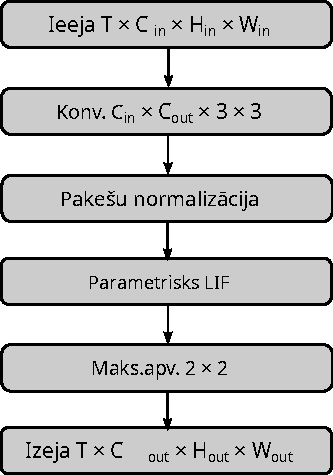
\includegraphics[width=0.25\linewidth]{fig/lv/layer_slice.pdf}
    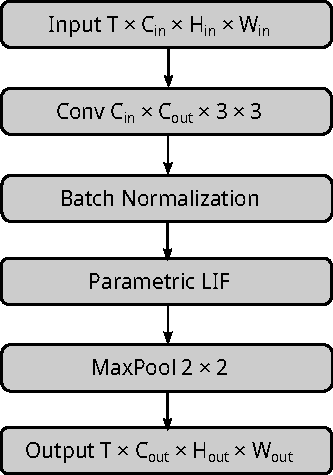
\includegraphics[width=0.25\linewidth]{fig/layer_slice.pdf}
    \caption{Impulsu konvolūcijas pamatbloks, kas sastāv no konvolūcijas, pakešu normalizācijas, LIF neirona un maksimuma apvienošanas operācijas.}
    \label{fig:spiking_conv_block}
\end{figure}

Apmācības laikā pēc konvolūcijām piemēro pakešu normalizāciju, lai uzlabotu zuduma funkcijas optimizāciju un stabilizētu aktivāciju sadalījumu tīklā \cite{ioffe2015}. Inferences laikā pakešu normalizācijas parametri tiek apvienoti ar konvolūcijas slāni, tādēļ aparatūras realizācijai nav nepieciešams atsevišķs normalizācijas slānis.

Pēc pakešu normalizācijas slāņiem seko \Gls{lif} impulsu neironu slāņi \cite{Fang2021}. Šajā darbā izmantoti adaptīvi \Gls{lif} neironi. Uzlabojot tradicionālos \Gls{lif} neironus ar fiksētiem parametriem, membrānas laika konstante tiek apgūta apmācības laikā. Membrānas stāvokli var izteikt šādi \cite{Fang2021}:
\begin{equation}
    U[t] = \beta U[t-1](1-S[t-1]) + I[t],
\end{equation}
kur \(\beta\) ir apmācāms membrānas dilšanas parametrs, \(I[t]\) ir sinaptiskā ieeja un \(S[t]\) ir izejas impulss. Parametra \(\beta\) apmācība ļauj atsevišķiem neironiem pielāgot temporālās integrēšanas īpašības ieejas datu telpiski temporālajām īpašībām.

Līdzīgi kā tradicionālajos \Gls{cnn}, pēc impulsu neironu slāņiem seko maksimuma apvienošanas operācijas \cite{Fang2021}, lai samazinātu dimensijas un iegūtu galvenās pazīmes no impulsu virknēm.

Pamattīklam tiek pievienoti papildus konvolūcijas slāņi, kas pakāpeniski samazina telpisko izšķirtspēju un ģenerē vairāku
mērogu pazīmju kartes, līdzīgi kā \Gls{ssd} arhitektūrās \cite{liu2016}. Šos papildu slāņus izmanto objektu detektēšanai
dažādos mērogos, nodrošinot pazīmju reprezentācijas ar dažādiem uztveres laukiem.


